\scanpage{44}

\uline{1)} Soit $G$ groupe fini d'automorphismes d'un anneau \unsure{semi-local} $O$.
$G$ est transitif sur les idéaux maximaux $\underline m$, soit $G_d$ le stabilisateur de $\underline m_0$, et $G_i\subset G_d$ l'ens des \unsure{éléments} de $G_d$ qui définissent l'automorphisme identique de $O/\underline m$.
Sous ces conditions

a) Il existe $x\in O^{G_i}$ tel que $T_{G/G_i}x=1$. Donc pour $\unsure{\forall}$ $G$-$O$-modules $M$, on a
\[
\widehat H(G,M)=\widehat H(G_i,M)^{G/G_i}.
\]
\unsure{Doute|D'autre} pour qu'on ait $1\in T_G O$, i.e. $\widehat H(G,M)=0$ $\forall$ $M$, il f. et s. que $[G_i:e]$ ne soit pas multiple de la caractéristique $p$ de $O/\underline m$.

b) Si $G_i=\{e\}$, on a $H^1(G,O^*)=\{e\}$.

Plus généralement, quel que soit $G_i$, l'hom naturel
\[
H^1(G,O^*)\longrightarrow H^1\bigl(G_i,(\underline O^{\deleted{\unsure{G}}}/m)^*\bigr)
\]
est bijectif (?). Qu'en est-il dans le cas \deleted{$\unsure{G}$} des $\operatorname{Gl}(n,\underline O)$ au lieu de $\unsure{O^\times|O^*}$ ?
\margin{?}
\figure{\begin{tikzpicture}\draw (0,0)--(0,-1.25);\end{tikzpicture}}

Dans a, \unsure{entre}
\[
\begin{aligned}
\underbrace{\overline{\widehat H(G,M)}=\widehat H(G,\overline M)}_{\substack{\text{\unsure{justification}}\\\text{par Zariski;}\\\text{il y a des}\\\text{hyp. \unsure{noethériennes}}\\\text{à faire ??}}}
&=\widehat H\left(G,\bigoplus_{s\in G/G_d}s.\overline M_{\underline m_0}\right)
=\widehat H(G_d,\overline M_{\underline m_0})\\
&=\overline{H(G_d,M_{\underline m_0})}.
\end{aligned}
\]
\margin{dans le cas où $O$ est de dim $1$,\par \unsure{car} \unsure{annule} $\widehat H(G,M)$ !}
\figure{\begin{tikzpicture}\draw (0,0)--(0,-1.7);\end{tikzpicture}}

Considérons alors le diagramme :
\diagram{\begin{tikzcd}[column sep=large,row sep=large]
\widehat H(G,M)\arrow[r,"\sim"]\arrow[d,"\unsure{\sim}"'] & \widehat H(G_i,M)_{\deleted{\unsure{\underline m_0}}}^{G/G_i}\arrow[r,"\unsure{\mathrm{inj}}","\alpha"'] & \widehat H(G_i,M_{\underline m_0})^{G_d/G_i}\\
\widehat H(G_d,M)^{G/G_d}\arrow[rr,"\beta"] & & \widehat H(G_d,M_{\underline m_0})\simeq\widehat H(G_d,M)_{O_d-m_0O_d}\arrow[u,"\unsure{\sim}"']
\end{tikzcd}}
\margin{$\alpha$ et $\beta$ sont injectifs ; images denses}
\margin{on passe au quotient !}
\figure{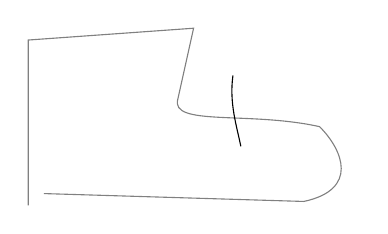
\begin{tikzpicture}[x=1cm,y=1cm]
\draw[gray] (0,-2.1)--(0,0)--(2.1,.15)--(1.9,-.75).. controls (1.8,-1.1) and (2.8,-.9)..(3.7,-1.1).. controls (4,-1.4) and (4.2,-1.9)..(3.5,-2.05)--(.2,-1.95);
\draw (2.6,-.45).. controls (2.55,-.8) and (2.65,-1.1)..(2.7,-1.35);
\end{tikzpicture}}

\mspage{43}

